\section{Noise Generation}
\label{section:noise}
Nature's chaotic and fortuitous behavior creates a world full of diversity and unpredictability.
This can be observed in a surprisingly high amount of objects, structures and phenomenons.
\\
For example, the following images show photographs of patterns that seem almost completely random.

\begin{figure}[H]
    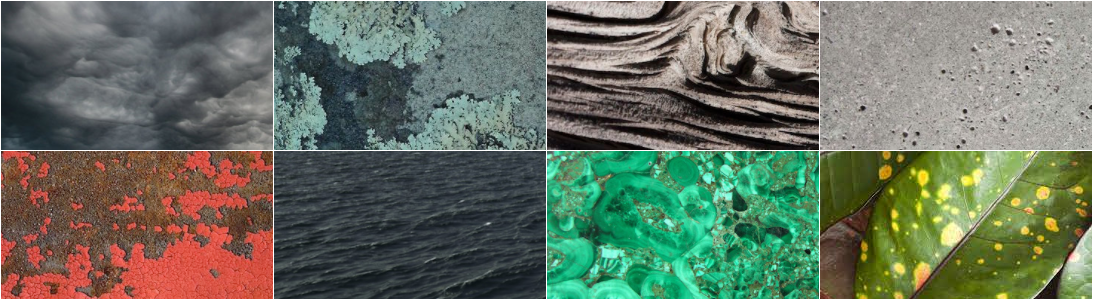
\includegraphics[width=\linewidth]{nature-random.png}
    \caption{Random pattern observed in Nature \protect\cite{bookofshaders:noise}.}
    \label{img:rnd:natural}
\end{figure}

\noindent
In computer science, the virtual recreation of such randomness has been studied continuously over the last decades.
The outcome of a randomness generator is called \emph{\gls{noise}}.
There are many established algorithms to create random patterns, one of which generates the famous \emph{Voronoi} \gls{noise}.

\subsection{Previous Work}
Many of the following subsections rely on concepts and algorithms that have been thorougly explained in the project's previous work \cite{project2:noise}.
This include sine-based deterministic number generation algorithms, also known as also \emph{\gls{pseudorandom}} number generation \cite{project2:noise:pseudo}.
It further includes different \gls{noisegeneration} algorithms like Perlin \gls{noise} \cite{project2:noise:perlin}.
\emptyline
Those algorithms will not be described again, as they have already been studied and documented before.

\pagebreak

\subsection{Voronoi Noise Algorithm}
\label{section:noise:voronoi}
One of the more commonly used procedural pattern generation algorithms is that of Steven Worley, developed in 1996 \cite{worley}, called \emph{Worley}'s algorithm.
The algorithm is also known as the \emph{Voronoi} algorithm due to its similar appearance to a Voronoi diagram.
In that diagram, points, called \emph{seeds}, are randomly scattered inside a defined space.
After that, regions are created, consisting of all points closer to that seed than to any other.
\\
The Voronoi \gls{noise} algorithm creates a cellular pattern and is therefore well suited for simulating natural distribution of cloud heaps, as they are in some way also arranged in cells.
\emptyline
The \gls{noise} algorithm starts by dividing the space into a grid, for which each cell is assigned a random point.
From there, each fragment gets shaded by how far it is to the seed in its cell.

\begin{figure}[H]
    \centering

    \begin{minipage}{0.47\linewidth}
        \centering
        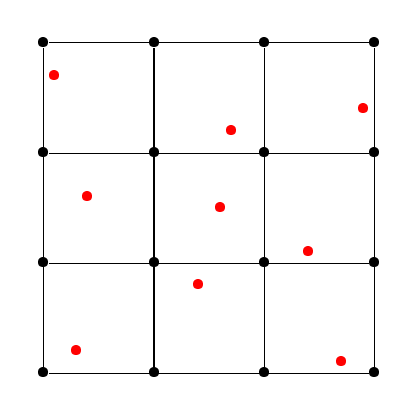
\begin{tikzpicture}[scale=0.7, x=2cm,y=2cm]
        \tikzset{c/.style = {shorten <=-4pt, shorten >=-4pt}}
        \tikzset{smalledge/.style = {-{Latex[length=2mm]},shorten <=-4pt}}
        
        \node (x1y1) at (0,0) {\textbullet};
        \node (x2y1) at (1,0) {\textbullet};
        \node (x3y1) at (2,0) {\textbullet};
        \node (x4y1) at (3,0) {\textbullet};

        \node (x1y2) at (0,1) {\textbullet};
        \node (x2y2) at (1,1) {\textbullet};
        \node (x3y2) at (2,1) {\textbullet};
        \node (x4y2) at (3,1) {\textbullet};

        \node (x1y3) at (0,2) {\textbullet};
        \node (x2y3) at (1,2) {\textbullet};
        \node (x3y3) at (2,2) {\textbullet};
        \node (x4y3) at (3,2) {\textbullet};

        \node (x1y4) at (0,3) {\textbullet};
        \node (x2y4) at (1,3) {\textbullet};
        \node (x3y4) at (2,3) {\textbullet};
        \node (x4y4) at (3,3) {\textbullet};

        \draw[c] (x1y1) edge node{} (x4y1);
        \draw[c] (x1y2) edge node{} (x4y2);
        \draw[c] (x1y3) edge node{} (x4y3);
        \draw[c] (x1y4) edge node{} (x4y4);

        \draw[c] (x1y1) edge node{} (x1y4);
        \draw[c] (x2y1) edge node{} (x2y4);
        \draw[c] (x3y1) edge node{} (x3y4);
        \draw[c] (x4y1) edge node{} (x4y4);

        \node[red] (s1) at (0.3,0.2) {\textbullet};
        \node[red] (s2) at (1.4,0.8) {\textbullet};
        \node[red] (s3) at (2.7,0.1) {\textbullet};
        \node[red] (s4) at (0.4,1.6) {\textbullet};
        \node[red] (s5) at (1.6,1.5) {\textbullet};
        \node[red] (s6) at (2.4,1.1) {\textbullet};
        \node[red] (s7) at (0.1,2.7) {\textbullet};
        \node[red] (s8) at (1.7,2.2) {\textbullet};
        \node[red] (s9) at (2.9,2.4) {\textbullet};

        \end{tikzpicture}
        \captionof{figure}{Voronoi grid with \gls{pseudorandom}ly assigned seed points for each cell.}
        \label{img:tikz:noise:voronoi}
    \end{minipage}
    \hfill
    \begin{minipage}{0.47\linewidth}
        \centering
        \begin{tikzpicture}[scale=0.7, x=2cm,y=2cm]
            \tikzset{c/.style = {shorten <=-4pt, shorten >=-4pt}}
            \tikzset{smalledge/.style = {-{Latex[length=2mm]},shorten <=-4pt}}
            
            \node (gradient) at (1.5,1.5) {
\includegraphics[width=4.2cm] {noise/2d voronoi unmixed}};

            \node (x1y1) at (0,0) {\textbullet};
            \node (x2y1) at (1,0) {\textbullet};
            \node (x3y1) at (2,0) {\textbullet};
            \node (x4y1) at (3,0) {\textbullet};

            \node (x1y2) at (0,1) {\textbullet};
            \node (x2y2) at (1,1) {\textbullet};
            \node (x3y2) at (2,1) {\textbullet};
            \node (x4y2) at (3,1) {\textbullet};

            \node (x1y3) at (0,2) {\textbullet};
            \node (x2y3) at (1,2) {\textbullet};
            \node (x3y3) at (2,2) {\textbullet};
            \node (x4y3) at (3,2) {\textbullet};

            \node (x1y4) at (0,3) {\textbullet};
            \node (x2y4) at (1,3) {\textbullet};
            \node (x3y4) at (2,3) {\textbullet};
            \node (x4y4) at (3,3) {\textbullet};

            \draw[c] (x1y1) edge node{} (x4y1);
            \draw[c] (x1y2) edge node{} (x4y2);
            \draw[c] (x1y3) edge node{} (x4y3);
            \draw[c] (x1y4) edge node{} (x4y4);

            \draw[c] (x1y1) edge node{} (x1y4);
            \draw[c] (x2y1) edge node{} (x2y4);
            \draw[c] (x3y1) edge node{} (x3y4);
            \draw[c] (x4y1) edge node{} (x4y4);

            \node[red] (s1) at (0.3,0.2) {\textbullet};
            \node[red] (s2) at (1.4,0.8) {\textbullet};
            \node[red] (s3) at (2.7,0.1) {\textbullet};
            \node[red] (s4) at (0.4,1.6) {\textbullet};
            \node[red] (s5) at (1.6,1.5) {\textbullet};
            \node[red] (s6) at (2.4,1.1) {\textbullet};
            \node[red] (s7) at (0.1,2.7) {\textbullet};
            \node[red] (s8) at (1.7,2.2) {\textbullet};
            \node[red] (s9) at (2.9,2.4) {\textbullet};

        \end{tikzpicture}
        \captionof{figure}{Voronoi grid with seed distances visualized.}
        \label{img:tikz:noise:voronoi2}
    \end{minipage}
\end{figure}

\noindent
As reckognizable in \autoref{img:tikz:noise:voronoi2}, hard contours are still visible along the grid lines. This can be improved by including the adjacent cells when finding the closest seed for any given fragment.
This amounts to $3^n - 1$ neighboring cells, where $n$ is the number of dimensions. This means for 2D space its eight cells, while in 3D its 26.

\begin{figure}[H]
    \centering
    \begin{tikzpicture}[scale=1.2, x=2cm,y=2cm]
        \tikzset{c/.style = {shorten <=-4pt, shorten >=-4pt}}
        \tikzset{smalledge/.style = {-{Latex[length=2mm]},shorten <=-4pt}}
        
        \node (gradient) at (1.5,1.5) {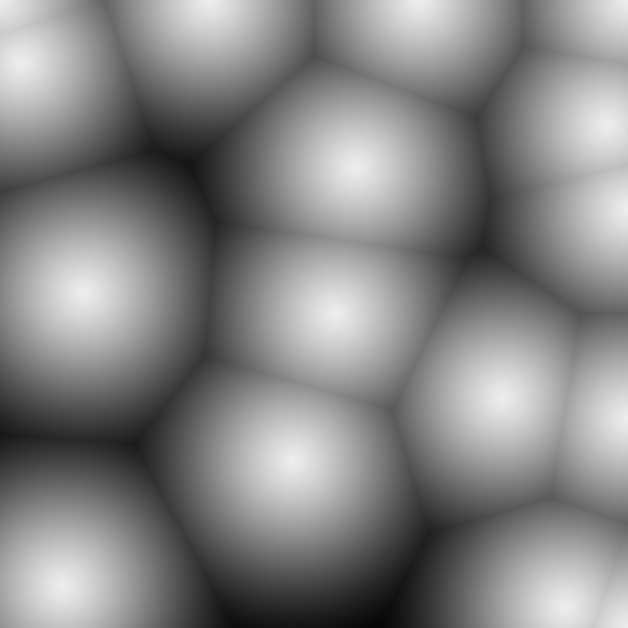
\includegraphics[width=7.2cm] {noise/2d voronoi}};

        \node (x1y1) at (0,0) {\textbullet};
        \node (x2y1) at (1,0) {\textbullet};
        \node (x3y1) at (2,0) {\textbullet};
        \node (x4y1) at (3,0) {\textbullet};

        \node (x1y2) at (0,1) {\textbullet};
        \node (x2y2) at (1,1) {\textbullet};
        \node (x3y2) at (2,1) {\textbullet};
        \node (x4y2) at (3,1) {\textbullet};

        \node (x1y3) at (0,2) {\textbullet};
        \node (x2y3) at (1,2) {\textbullet};
        \node (x3y3) at (2,2) {\textbullet};
        \node (x4y3) at (3,2) {\textbullet};

        \node (x1y4) at (0,3) {\textbullet};
        \node (x2y4) at (1,3) {\textbullet};
        \node (x3y4) at (2,3) {\textbullet};
        \node (x4y4) at (3,3) {\textbullet};

        \draw[c] (x1y1) edge node{} (x4y1);
        \draw[c] (x1y2) edge node{} (x4y2);
        \draw[c] (x1y3) edge node{} (x4y3);
        \draw[c] (x1y4) edge node{} (x4y4);

        \draw[c] (x1y1) edge node{} (x1y4);
        \draw[c] (x2y1) edge node{} (x2y4);
        \draw[c] (x3y1) edge node{} (x3y4);
        \draw[c] (x4y1) edge node{} (x4y4);

        \node[red] (s1) at (0.3,0.2) {\textbullet};
        \node[red] (s2) at (1.4,0.8) {\textbullet};
        \node[red] (s3) at (2.7,0.1) {\textbullet};
        \node[red] (s4) at (0.4,1.6) {\textbullet};
        \node[red] (s5) at (1.6,1.5) {\textbullet};
        \node[red] (s6) at (2.4,1.1) {\textbullet};
        \node[red] (s7) at (0.1,2.7) {\textbullet};
        \node[red] (s8) at (1.7,2.2) {\textbullet};
        \node[red] (s9) at (2.9,2.4) {\textbullet};

    \end{tikzpicture}
    \captionof{figure}{Complete 2D Voronoi \gls{noise} texture.}
    \label{img:tikz:noise:voronoi3}
\end{figure}

\pagebreak

\noindent
An implementation of this relatively simple algorithm could look like the following listing.
\begin{lstlisting}[language=HLSL, caption=Implementation of 2D Voronoi \gls{noise} algorithm., label=lst:shader:noise:voronoi2d]
float2 randomSeed(float2 co) {
    return float2(
        fract(sin(dot(co, float2(12.9898, 78.233))) * 43758.5453123),
        fract(sin(dot(co, float2(39.3461, 11.135))) * 14375.8545359));
}

float voronoi(float2 p) {
    float2 baseCell = floor(p);
    float dMin = 999;

    for(int x = -1; x <= 1; x++) {
        for(int y = -1; y <= 1; y++) {
            float2 cell = baseCell + float2(x, y);
            float2 seed = cell + randomSeed(cell);
            float d = distance(seed, p);
            if (d < dMin) {
                dMin = d;
            }
        }
    }
    return dMin;
}
\end{lstlisting}

\noindent
The 3D equivalent of the algorithm looks fairly similar.

\begin{lstlisting}[language=HLSL, caption=Implementation of 3D Voronoi \gls{noise} algorithm., label=lst:shader:noise:voronoi3d]
float3 randomSeed(float3 co) {
    return float3(
    fract(sin(dot(co, float3(12.989, 78.233, 37.719))) * 43758.5453123),
    fract(sin(dot(co, float3(39.346, 11.135, 83.155))) * 14375.8545346),
    fract(sin(dot(co, float3(73.156, 52.235, 09.151))) * 31396.2234116));
}

float voronoi(float3 p) {
    float3 baseCell = floor(p);
    float dMin = 999;

    for(int x = -1; x <= 1; x++) {
        for(int y = -1; y <= 1; y++) {
            for(int z = -1; z <= 1; z++) {
                float3 cell = baseCell + float3(x, y, z);
                float3 seed = cell + randomSeed(cell);
                float d = distance(seed, p);
                if (d < dMin) {
                    dMin = d;
                }
            }
        }
    }
    return dMin;
}
\end{lstlisting}

\subsection{Seamless Noise}
\label{section:noise:seamless}
In \autoref{img:tikz:noise:voronoi3}, the generated cells appear to be randomly distributed, but there is still a major flaw in the texture.
\\
As already mentioned previously, the \gls{noisegeneration} is confined to a fixed region.
This poses an issue when the desired area is larger than the defined space of the algorithm.
It is therefore not possible to tile the same texture without visible seams inbetween the tiles.

\begin{figure}[H]
    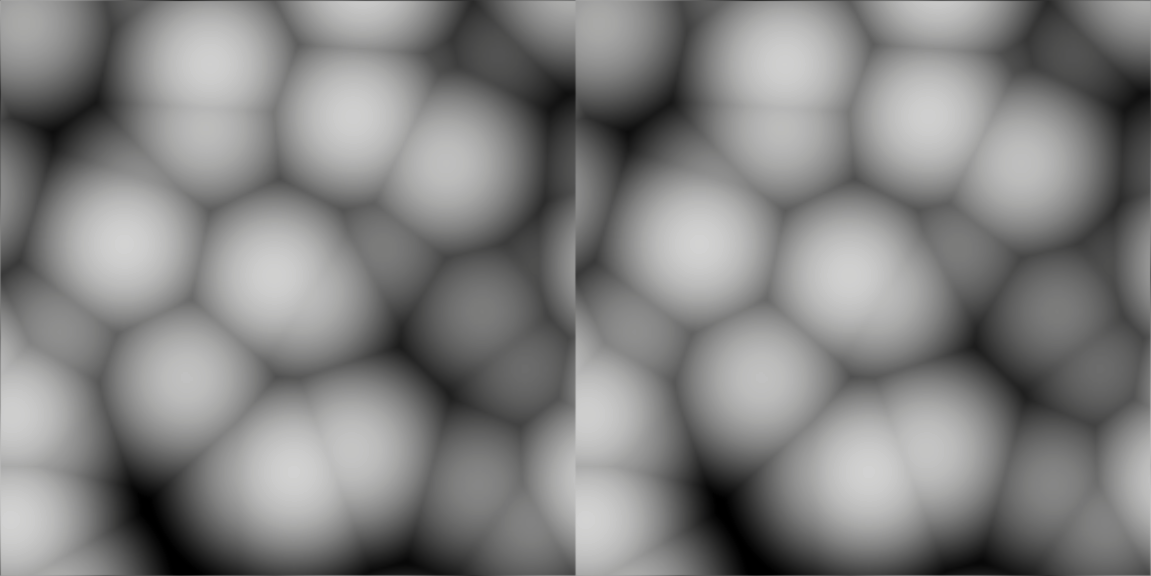
\includegraphics[width=\linewidth]{noise/voronoi seam.png}
    \caption{Tiled 3D \gls{noise} \gls{textureslice}s.}
    \label{img:rnd:noise:seam}
\end{figure}

\noindent
The problem occurs when checking the neighboring cells of the current cell. For example, here are the seeds for two adjacent tiles of the same \gls{noise} texture.

\begin{figure}[H]
    \centering
    \begin{tikzpicture}[scale=0.9, x=2cm,y=2cm]
    \tikzset{c/.style = {shorten <=-4pt, shorten >=-4pt}}
    \tikzset{smalledge/.style = {-{Latex[length=2mm]},shorten <=-4pt}}
    
    % tile label 1
    \draw (0,3.3) -- (3,3.3);
    \draw (0,3.25) -- (0,3.35);
    \draw (3,3.25) -- (3,3.35);
    \node at (1.5,3.4) {first tile};
    
    % tile label 2
    \draw (3,-0.3) -- (6,-0.3);
    \draw (3,-0.25) -- (3,-0.35);
    \draw (6,-0.25) -- (6,-0.35);
    \node at (4.5,-0.4) {second tile};

    \node (offset) at (3.0,0) {};

    \fill[cyan!5] (offset) rectangle ($(offset) + (3,3)$);
    \fill[red!5] (0,0) rectangle (3,3);

    \node (x1y1) at (0,0) {\textbullet};
    \node (x2y1) at (1,0) {\textbullet};
    \node (x3y1) at (2,0) {\textbullet};
    \node (x4y1) at (3,0) {\textbullet};

    \node (x1y2) at (0,1) {\textbullet};
    \node (x2y2) at (1,1) {\textbullet};
    \node (x3y2) at (2,1) {\textbullet};
    \node (x4y2) at (3,1) {\textbullet};

    \node (x1y3) at (0,2) {\textbullet};
    \node (x2y3) at (1,2) {\textbullet};
    \node (x3y3) at (2,2) {\textbullet};
    \node (x4y3) at (3,2) {\textbullet};

    \node (x1y4) at (0,3) {\textbullet};
    \node (x2y4) at (1,3) {\textbullet};
    \node (x3y4) at (2,3) {\textbullet};
    \node (x4y4) at (3,3) {\textbullet};

    \draw[c] (x1y1) edge node{} (x4y1);
    \draw[c] (x1y2) edge node{} (x4y2);
    \draw[c] (x1y3) edge node{} (x4y3);
    \draw[c] (x1y4) edge node{} (x4y4);

    \draw[c] (x1y1) edge node{} (x1y4);
    \draw[c] (x2y1) edge node{} (x2y4);
    \draw[c] (x3y1) edge node{} (x3y4);
    \draw[c] (x4y1) edge node{} (x4y4);

    \node[red] (s1) at (0.3,0.2) {\textbullet};
    \node[red] (s2) at (1.4,0.8) {\textbullet};
    \node[red] (s3) at (2.7,0.1) {\textbullet};
    \node[red] (s4) at (0.4,1.6) {\textbullet};
    \node[red] (s5) at (1.6,1.5) {\textbullet};
    \node[red] (s6) at (2.4,1.1) {\textbullet};
    \node[red] (s7) at (0.1,2.7) {\textbullet};
    \node[red] (s8) at (1.7,2.2) {\textbullet};
    \node[red] (s9) at (2.9,2.4) {\textbullet};

    \node (x1y1) at ($(offset) + (0,0)$) {};
    \node (x2y1) at ($(offset) + (1,0)$) {\textbullet};
    \node (x3y1) at ($(offset) + (2,0)$) {\textbullet};
    \node (x4y1) at ($(offset) + (3,0)$) {\textbullet};

    \node (x1y2) at ($(offset) + (0,1)$) {};
    \node (x2y2) at ($(offset) + (1,1)$) {\textbullet};
    \node (x3y2) at ($(offset) + (2,1)$) {\textbullet};
    \node (x4y2) at ($(offset) + (3,1)$) {\textbullet};

    \node (x1y3) at ($(offset) + (0,2)$) {};
    \node (x2y3) at ($(offset) + (1,2)$) {\textbullet};
    \node (x3y3) at ($(offset) + (2,2)$) {\textbullet};
    \node (x4y3) at ($(offset) + (3,2)$) {\textbullet};

    \node (x1y4) at ($(offset) + (0,3)$) {};
    \node (x2y4) at ($(offset) + (1,3)$) {\textbullet};
    \node (x3y4) at ($(offset) + (2,3)$) {\textbullet};
    \node (x4y4) at ($(offset) + (3,3)$) {\textbullet};

    \draw[c] (x1y1) edge node{} (x4y1);
    \draw[c] (x1y2) edge node{} (x4y2);
    \draw[c] (x1y3) edge node{} (x4y3);
    \draw[c] (x1y4) edge node{} (x4y4);

    \draw[c] (x2y1) edge node{} (x2y4);
    \draw[c] (x3y1) edge node{} (x3y4);
    \draw[c] (x4y1) edge node{} (x4y4);

    \node[cyan] (s1) at ($(offset) + (0.8,0.8)$) {\textbullet};
    \node[cyan] (s2) at ($(offset) + (1.7,0.2)$) {\textbullet};
    \node[cyan] (s3) at ($(offset) + (2.1,0.6)$) {\textbullet};
    \node[cyan] (s4) at ($(offset) + (0.2,1.4)$) {\textbullet};
    \node[cyan] (s5) at ($(offset) + (1.2,1.8)$) {\textbullet};
    \node[cyan] (s6) at ($(offset) + (2.7,1.4)$) {\textbullet};
    \node[cyan] (s7) at ($(offset) + (0.3,2.1)$) {\textbullet};
    \node[cyan] (s8) at ($(offset) + (1.7,2.4)$) {\textbullet};
    \node[cyan] (s9) at ($(offset) + (2.2,2.5)$) {\textbullet};

    \end{tikzpicture}
    \captionof{figure}{Voronoi \gls{noise} seeds of the second tile are different than the seeds of the first tile.}
    \label{img:tikz:noise:seamless:1}
\end{figure}

\pagebreak

\noindent
When inspecting the cell $c_{2,1}$ of the first tile, some of its neighbors, namely $c_{3,0}$ to $c_{3,2}$, are part of the next tile.
However, since the desired outcome is a repeating texture, the underlaying texture will be the same as the first one.

\begin{figure}[H]
    \centering
    \begin{tikzpicture}[scale=0.9, x=2cm,y=2cm]
    \tikzset{c/.style = {shorten <=-4pt, shorten >=-4pt}}
    \tikzset{smalledge/.style = {-{Latex[length=2mm]},shorten <=-4pt}}
    
    % tile label 1
    \draw (0,3.3) -- (3,3.3);
    \draw (0,3.25) -- (0,3.35);
    \draw (3,3.25) -- (3,3.35);
    \node at (1.5,3.4) {first tile};
    
    % tile label 2
    \draw (3,-0.3) -- (6,-0.3);
    \draw (3,-0.25) -- (3,-0.35);
    \draw (6,-0.25) -- (6,-0.35);
    \node at (4.5,-0.4) {second tile};

    \node (offset) at (3.0,0) {};

    \fill[cyan!5] (offset) rectangle ($(offset) + (1,3)$);
    \fill[red!5] (1,0) rectangle (3,3);

    \node[black!20] (x1y1) at (0,0) {\textbullet};
    \node (x2y1) at (1,0) {\textbullet};
    \node (x3y1) at (2,0) {\textbullet};
    \node (x4y1) at (3,0) {\textbullet};

    \node[black!20] (x1y2) at (0,1) {\textbullet};
    \node (x2y2) at (1,1) {\textbullet};
    \node (x3y2) at (2,1) {\textbullet};
    \node (x4y2) at (3,1) {\textbullet};

    \node[black!20] (x1y3) at (0,2) {\textbullet};
    \node (x2y3) at (1,2) {\textbullet};
    \node (x3y3) at (2,2) {\textbullet};
    \node (x4y3) at (3,2) {\textbullet};

    \node[black!20] (x1y4) at (0,3) {\textbullet};
    \node (x2y4) at (1,3) {\textbullet};
    \node (x3y4) at (2,3) {\textbullet};
    \node (x4y4) at (3,3) {\textbullet};

    \draw[c,black!20] (x1y1) edge node{} (x2y1);
    \draw[c,black!20] (x1y2) edge node{} (x2y2);
    \draw[c,black!20] (x1y3) edge node{} (x2y3);
    \draw[c,black!20] (x1y4) edge node{} (x2y4);
    \draw[c] (x2y1) edge node{} (x4y1);
    \draw[c] (x2y2) edge node{} (x4y2);
    \draw[c] (x2y3) edge node{} (x4y3);
    \draw[c] (x2y4) edge node{} (x4y4);

    \draw[c,black!20] (x1y1) edge node{} (x1y4);
    \draw[c] (x2y1) edge node{} (x2y4);
    \draw[c] (x3y1) edge node{} (x3y4);
    \draw[c] (x4y1) edge node{} (x4y4);

    \node[red!20] (s1) at (0.3,0.2) {\textbullet};
    \node[red] (s2) at (1.4,0.8) {\textbullet};
    \node[red] (s3) at (2.7,0.1) {\textbullet};
    \node[red!20] (s4) at (0.4,1.6) {\textbullet};
    \node[red] (s5) at (1.6,1.5) {\textbullet};
    \node[red] (s6) at (2.4,1.1) {\textbullet};
    \node[red!20] (s7) at (0.1,2.7) {\textbullet};
    \node[red] (s8) at (1.7,2.2) {\textbullet};
    \node[red] (s9) at (2.9,2.4) {\textbullet};

    \node (x1y1) at ($(offset) + (0,0)$) {};
    \node (x2y1) at ($(offset) + (1,0)$) {\textbullet};
    \node[black!20] (x3y1) at ($(offset) + (2,0)$) {\textbullet};
    \node[black!20] (x4y1) at ($(offset) + (3,0)$) {\textbullet};

    \node (x1y2) at ($(offset) + (0,1)$) {};
    \node (x2y2) at ($(offset) + (1,1)$) {\textbullet};
    \node[black!20] (x3y2) at ($(offset) + (2,1)$) {\textbullet};
    \node[black!20] (x4y2) at ($(offset) + (3,1)$) {\textbullet};

    \node (x1y3) at ($(offset) + (0,2)$) {};
    \node (x2y3) at ($(offset) + (1,2)$) {\textbullet};
    \node[black!20] (x3y3) at ($(offset) + (2,2)$) {\textbullet};
    \node[black!20] (x4y3) at ($(offset) + (3,2)$) {\textbullet};

    \node (x1y4) at ($(offset) + (0,3)$) {};
    \node (x2y4) at ($(offset) + (1,3)$) {\textbullet};
    \node[black!20] (x3y4) at ($(offset) + (2,3)$) {\textbullet};
    \node[black!20] (x4y4) at ($(offset) + (3,3)$) {\textbullet};

    \draw[c] (x1y1) edge node{} (x2y1);
    \draw[c] (x1y2) edge node{} (x2y2);
    \draw[c] (x1y3) edge node{} (x2y3);
    \draw[c] (x1y4) edge node{} (x2y4);
    \draw[c,black!20] (x2y1) edge node{} (x4y1);
    \draw[c,black!20] (x2y2) edge node{} (x4y2);
    \draw[c,black!20] (x2y3) edge node{} (x4y3);
    \draw[c,black!20] (x2y4) edge node{} (x4y4);

    \draw[c] (x2y1) edge node{} (x2y4);
    \draw[c,black!20] (x3y1) edge node{} (x3y4);
    \draw[c,black!20] (x4y1) edge node{} (x4y4);

    \node[cyan] (s1) at ($(offset) + (0.8,0.8)$) {\textbullet};
    \node[cyan!20] (s2) at ($(offset) + (1.7,0.2)$) {\textbullet};
    \node[cyan!20] (s3) at ($(offset) + (2.1,0.6)$) {\textbullet};
    \node[cyan] (s4) at ($(offset) + (0.2,1.4)$) {\textbullet};
    \node[cyan!20] (s5) at ($(offset) + (1.2,1.8)$) {\textbullet};
    \node[cyan!20] (s6) at ($(offset) + (2.7,1.4)$) {\textbullet};
    \node[cyan] (s7) at ($(offset) + (0.3,2.1)$) {\textbullet};
    \node[cyan!20] (s8) at ($(offset) + (1.7,2.4)$) {\textbullet};
    \node[cyan!20] (s9) at ($(offset) + (2.2,2.5)$) {\textbullet};

    % cell label
    \node[anchor=west] at (2.05,1.85) {$c_{2,1}$};
    \node[black!70,anchor=west] at (3.05,0.85) {$c_{3,0}$};
    \node[black!70,anchor=west] at (3.05,1.85) {$c_{3,1}$};
    \node[black!70,anchor=west] at (3.05,2.85) {$c_{3,2}$};
    \draw[line width=0.6mm] (2,1) -- (3,1) -- (3,2) -- (2,2) -- (2,1);

    \end{tikzpicture}
    \captionof{figure}{Voronoi \gls{noise} seeds are sampled from the second tile.}
    \label{img:tikz:noise:seamless:2}
\end{figure}

\noindent
Naturally, when using seeds from the second tile but placing the texture from the first tile underneath, a disruption in the pattern will be visible in the form of a seam.
This is why, when the sampling point exceeds the defined space of the texture, the seeds will always be calculated based on the first tile again.
Instead of sampling $c_{3,0}$ to $c_{3,2}$ from the second tile, $c_{0,0}$ to $c_{0,2}$ will be used.

\begin{figure}[H]
    \centering
    \begin{tikzpicture}[scale=0.9, x=2cm,y=2cm]
    \tikzset{c/.style = {shorten <=-4pt, shorten >=-4pt}}
    \tikzset{smalledge/.style = {-{Latex[length=2mm]},shorten <=-4pt}}
    
    % tile label 1
    \draw (0,3.3) -- (3,3.3);
    \draw (0,3.25) -- (0,3.35);
    \draw (3,3.25) -- (3,3.35);
    \node at (1.5,3.4) {first tile};
    
    % tile label 2
    \draw (3,-0.3) -- (6,-0.3);
    \draw (3,-0.25) -- (3,-0.35);
    \draw (6,-0.25) -- (6,-0.35);
    \node at (4.5,-0.4) {second tile};

    \node (offset) at (3.0,0) {};

    \fill[red!5] (0,0) rectangle (1,3);
    \fill[cyan!5] (3,0) rectangle (4,3);
    \fill[red!5] (2,1) rectangle (3,2);

    \node (x1y1) at (0,0) {\textbullet};
    \node (x2y1) at (1,0) {\textbullet};
    \node[black!20] (x3y1) at (2,0) {\textbullet};
    \node (x4y1) at (3,0) {\textbullet};

    \node (x1y2) at (0,1) {\textbullet};
    \node (x2y2) at (1,1) {\textbullet};
    \node[black!20] (x3y2) at (2,1) {\textbullet};
    \node (x4y2) at (3,1) {\textbullet};

    \node (x1y3) at (0,2) {\textbullet};
    \node (x2y3) at (1,2) {\textbullet};
    \node[black!20] (x3y3) at (2,2) {\textbullet};
    \node (x4y3) at (3,2) {\textbullet};

    \node (x1y4) at (0,3) {\textbullet};
    \node (x2y4) at (1,3) {\textbullet};
    \node[black!20] (x3y4) at (2,3) {\textbullet};
    \node (x4y4) at (3,3) {\textbullet};

    \draw[c] (x1y1) edge node{} (x2y1);
    \draw[c] (x1y2) edge node{} (x2y2);
    \draw[c] (x1y3) edge node{} (x2y3);
    \draw[c] (x1y4) edge node{} (x2y4);
    \draw[c,black!20] (x2y1) edge node{} (x4y1);
    \draw[c,black!20] (x2y2) edge node{} (x4y2);
    \draw[c,black!20] (x2y3) edge node{} (x4y3);
    \draw[c,black!20] (x2y4) edge node{} (x4y4);

    \draw[c] (x1y1) edge node{} (x1y4);
    \draw[c] (x2y1) edge node{} (x2y4);
    \draw[c,black!20] (x3y1) edge node{} (x3y4);
    \draw[c] (x4y1) edge node{} (x4y4);

    \node[red] (s1) at (0.3,0.2) {\textbullet};
    \node[red!20] (s2) at (1.4,0.8) {\textbullet};
    \node[red!20] (s3) at (2.7,0.1) {\textbullet};
    \node[red] (s4) at (0.4,1.6) {\textbullet};
    \node[red!20] (s5) at (1.6,1.5) {\textbullet};
    \node[red] (s6) at (2.4,1.1) {\textbullet};
    \node[red] (s7) at (0.1,2.7) {\textbullet};
    \node[red!20] (s8) at (1.7,2.2) {\textbullet};
    \node[red!20] (s9) at (2.9,2.4) {\textbullet};

    \node (x1y1) at ($(offset) + (0,0)$) {};
    \node (x2y1) at ($(offset) + (1,0)$) {\textbullet};
    \node[black!20] (x3y1) at ($(offset) + (2,0)$) {\textbullet};
    \node[black!20] (x4y1) at ($(offset) + (3,0)$) {\textbullet};

    \node (x1y2) at ($(offset) + (0,1)$) {};
    \node (x2y2) at ($(offset) + (1,1)$) {\textbullet};
    \node[black!20] (x3y2) at ($(offset) + (2,1)$) {\textbullet};
    \node[black!20] (x4y2) at ($(offset) + (3,1)$) {\textbullet};

    \node (x1y3) at ($(offset) + (0,2)$) {};
    \node (x2y3) at ($(offset) + (1,2)$) {\textbullet};
    \node[black!20] (x3y3) at ($(offset) + (2,2)$) {\textbullet};
    \node[black!20] (x4y3) at ($(offset) + (3,2)$) {\textbullet};

    \node (x1y4) at ($(offset) + (0,3)$) {};
    \node (x2y4) at ($(offset) + (1,3)$) {\textbullet};
    \node[black!20] (x3y4) at ($(offset) + (2,3)$) {\textbullet};
    \node[black!20] (x4y4) at ($(offset) + (3,3)$) {\textbullet};

    \draw[c] (x1y1) edge node{} (x2y1);
    \draw[c] (x1y2) edge node{} (x2y2);
    \draw[c] (x1y3) edge node{} (x2y3);
    \draw[c] (x1y4) edge node{} (x2y4);
    \draw[c,black!20] (x2y1) edge node{} (x4y1);
    \draw[c,black!20] (x2y2) edge node{} (x4y2);
    \draw[c,black!20] (x2y3) edge node{} (x4y3);
    \draw[c,black!20] (x2y4) edge node{} (x4y4);

    \draw[c] (x2y1) edge node{} (x2y4);
    \draw[c,black!20] (x3y1) edge node{} (x3y4);
    \draw[c,black!20] (x4y1) edge node{} (x4y4);

    \node[red] (s1) at ($(offset) + (0.3,0.2)$) {\textbullet};
    \node[cyan!20] (s2) at ($(offset) + (1.7,0.2)$) {\textbullet};
    \node[cyan!20] (s3) at ($(offset) + (2.1,0.6)$) {\textbullet};
    \node[red] (s4) at ($(offset) + (0.4,1.6)$) {\textbullet};
    \node[cyan!20] (s5) at ($(offset) + (1.2,1.8)$) {\textbullet};
    \node[cyan!20] (s6) at ($(offset) + (2.7,1.4)$) {\textbullet};
    \node[red] (s7) at ($(offset) + (0.1,2.7)$) {\textbullet};
    \node[cyan!20] (s8) at ($(offset) + (1.7,2.4)$) {\textbullet};
    \node[cyan!20] (s9) at ($(offset) + (2.2,2.5)$) {\textbullet};

    % cell label
    \node[anchor=west] at (2.05,1.85) {$c_{2,1}$};
    \node[black!70,anchor=west] at (0.05,0.85) {$c_{0,0}$};
    \node[black!70,anchor=west] at (0.05,1.85) {$c_{0,1}$};
    \node[black!70,anchor=west] at (0.05,2.85) {$c_{0,2}$};
    \node[black!70,anchor=west] at (3.05,0.85) {$c_{3,0}$};
    \node[black!70,anchor=west] at (3.05,1.85) {$c_{3,1}$};
    \node[black!70,anchor=west] at (3.05,2.85) {$c_{3,2}$};
    \draw[line width=0.6mm] (2,1) -- (3,1) -- (3,2) -- (2,2) -- (2,1);

    \end{tikzpicture}
    \captionof{figure}{Voronoi \gls{noise} seeds that exceed the boundary are sampled from the first set again.}
    \label{img:tikz:noise:seamless:3}
\end{figure}

\noindent
In conclusion, the same set of points that is calculated for the first texture tile needs to be used again for every succeeding tile.

\pagebreak

\noindent
Mathematically, this is solved by using the $modulo$ operation. The dividend is the current cell and the divisor is the period, or how often the \gls{noise} texture is repeated.

\begin{lstlisting}[language=HLSL, caption=Implementation of a partially seamless 3D Voronoi \gls{noise} algorithm., label=lst:shader:noise:voronoi:seamless1]
float voronoi(float3 p, float3 period) {
    float3 baseCell = floor(p);
    float dMin = 999;

    for(int x = -1; x <= 1; x++) {
        for(int y = -1; y <= 1; y++) {
            for(int z = -1; z <= 1; z++) {
                float3 cell = baseCell + float3(x, y, z);
                float3 tiledCell = cell % period;
                float3 seed = cell + randomSeed(tiledCell);
                float d = distance(seed, p);
                if (d < dMin) {
                    dMin = d;
                }
            }
        }
    }
    return dMin;
}
\end{lstlisting}

\noindent
Interestingly, this does only partially solve the problem. As it turns out, the modulo operation of the \gls{hlsl} treats negative values differently than expected.
Instead of returning the absolute modulo value, it returns the remainder, including negative values.
$$
\begin{array}{l}
    expected: -5 \bmod 3 = 1 \\
    \phantom{ex}actual: -5 \bmod 3 = -2
\end{array}
$$

\noindent
When used this way, the outcome still has visible seams where cell modulo operations has to deal with negative numbers.
The issue is further explained by Ronja \cite{ronja:tilingnoise}.

\begin{figure}[H]
    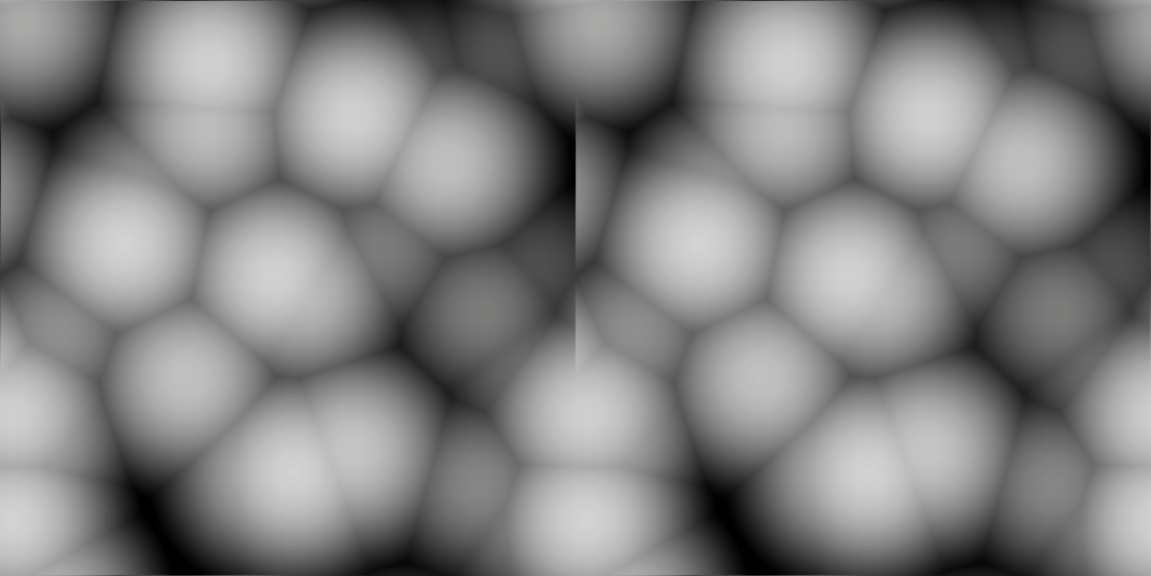
\includegraphics[width=\linewidth]{noise/voronoi seamless1.png}
    \caption{Partially seamless, tiled 3D \gls{noise} \gls{textureslice}s.}
    \label{img:rnd:noise:seamless1}
\end{figure}

\pagebreak

\noindent
The problem is easily fixed, though. To get a positive dividend, one can simply take the remainder of the dividend, add the divisor and then take the remainder again, knowing that the number will positive beforehand.
$$
\begin{array}{l}
    mod(x, y) = (x \mathbin{\%} y + y) \mathbin{\%} y
\end{array}
$$

\noindent
Alternatively, the implementation as described in the OpenGL documentation \cite{opengl:mod} can be used.
It is capable of dealing with negative dividends, and is defined as follows:
$$
\begin{array}{l}
    mod(x, y) = x - y * floor(x/y)
\end{array}
$$

\begin{lstlisting}[language=HLSL, caption=Implementation of seamless 3D Voronoi \gls{noise} algorithm., label=lst:shader:noise:voronoi:seamless2]
#define mod(x,y) (x-y*floor(x/y))

float voronoi(float3 p, float3 period) {
    float3 baseCell = floor(p);
    float dMin = 999;

    for(int x = -1; x <= 1; x++) {
        for(int y = -1; y <= 1; y++) {
            for(int z = -1; z <= 1; z++) {
                float3 cell = baseCell + float3(x, y, z);
                float3 tiledCell = mod(cell, period);
                float3 seed = cell + randomSeed(tiledCell);
                float d = distance(seed, p);
                if (d < dMin) {
                    dMin = d;
                }
            }
        }
    }
    return dMin;
}
\end{lstlisting}

\noindent
And with that, the \gls{noise} texture tiles seamlessly.

\begin{figure}[H]
    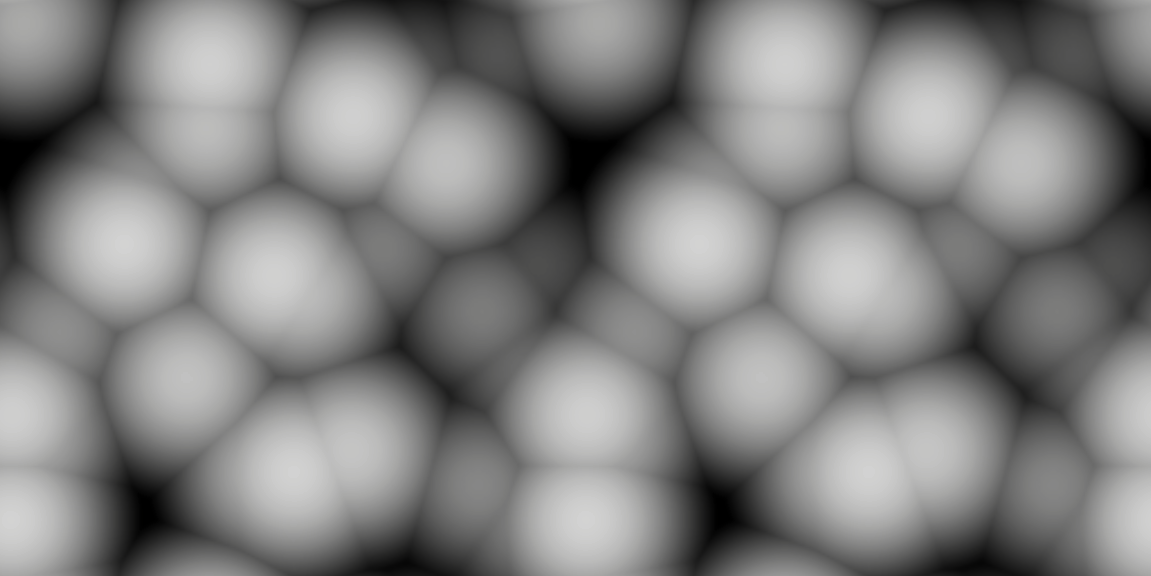
\includegraphics[width=\linewidth]{noise/voronoi seamless2.png}
    \caption{Seamlessly tiled 3D \gls{noise} \gls{textureslice}s.}
    \label{img:rnd:noise:seamless2}
\end{figure}

\subsection{Compute Shaders}
\label{section:noise:compute}
\Gls{computeshader}s are special programs that run on a graphics card. They are used for high-speed general-purpose computing.
Unlike regular \gls{shader}s, they do not write directly to the \gls{framebuffer}, but to a buffer from which the data can be read later on.
In many cases, this buffer is a 2D or 3D texture.

\subsubsection{Compute Shader Structure}
In Unity, compute shaders are written in \gls{hlsl} and interact with Microsoft's DirectCompute technology, a graphics card interface for \gls{computeshader}s.
This is a standard example of such a \gls{shader}:

\begin{lstlisting}[language=HLSL, caption=A standard \gls{computeshader} template., label=lst:shader:compute:standard]
#pragma kernel CSMain

RWTexture3D<float4> _Result;

[numthreads(4,4,4)]
void CSMain (uint3 id : SV_DispatchThreadID)
{
    _Result[id.xyz] = float4(1,0,0,1);
}
\end{lstlisting}

\noindent
The so-called \emph{\gls{kernel}} is defined on the first line and describes the method that will be executed when the \gls{computeshader} is dispatched.
In this example, there is only one \gls{kernel} with the name \lstinline[language=HLSL]{CSMain}.
When executed, it writes to a 3D texture and sets the color of a specific \gls{texel} (short for texture element) to red.
\\
On the third line, a 3D texture variable is declared.
The type is \lstinline[language=HLSL]{RWTexture3D}, which means the texture is enabled for both reading and writing.
Another important part is the \lstinline[language=HLSL]{[numthreads(8,8,8)]} statement. It specifies the dimensions of thread groups.

\subsubsection{Thread Groups}
When running a \gls{computeshader}, the kernel is executed on many threads in parallel.
This allows the \gls{gpu} to split up the computation instructions declared in the \gls{shader}.
For each part, a thread group is created, which only handles that specific part.
These thread groups run individually and simultaneously, speeding up the process massively.
\\
The dimensions of a thread group can be controlled with the \lstinline[language=HLSL]{numthreads} attribute.
In the example above, for each thread group, there will be 4 threads in the X dimension, 4 threads in the Y dimension and 4 threads in the Z dimension.
\emptyline
Every \gls{kernel} has a parameter called \lstinline[language=HLSL]{id}. This is the identifier of the current thread, short \emph{thread id}.
The thread id is unique for the whole execution. The following example shows how a thread group is structured.

\begin{figure}[H]
    \centering
    \begin{tikzpicture}[scale=0.6, x=2cm,y=2cm]
        \tikzset{c/.style = {shorten <=-4pt, shorten >=-4pt}}
        \tikzset{cb/.style = {shorten <=-4pt, shorten >=-4pt, black!30}}
        \tikzset{smalledge/.style = {-{Latex[length=2mm]},shorten <=-4pt,shorten >=-4pt}}
        
        \node (x1y1) at (0,0) {};
        \node (x1y2) at (0,1) {};
        \node (x1y3) at (0,2) {};
        \node (x1y4) at (0,3) {};
        \node (x1y5) at (0,4) {};
        
        \node (x2y1) at (1,0) {};
        \node (x2y5) at (1,4) {};
        
        \node (x3y1) at (2,0) {};
        \node (x3y5) at (2,4) {};
        
        \node (x4y1) at (3,0) {};
        \node (x4y5) at (3,4) {};
    
        \node (x5y1) at (4,0) {};
        \node (x5y2) at (4,1) {};
        \node (x5y3) at (4,2) {};
        \node (x5y4) at (4,3) {};
        \node (x5y5) at (4,4) {};
    
        \draw[c] (x1y1) edge node{} (x5y1);
        \draw[c] (x1y2) edge node{} (x5y2);
        \draw[c] (x1y3) edge node{} (x5y3);
        \draw[c] (x1y4) edge node{} (x5y4);
        \draw[c] (x1y5) edge node{} (x5y5);
    
        \draw[c] (x1y1) edge node{} (x1y5);
        \draw[c] (x2y1) edge node{} (x2y5);
        \draw[c] (x3y1) edge node{} (x3y5);
        \draw[c] (x4y1) edge node{} (x4y5);
        \draw[c] (x5y1) edge node{} (x5y5);
    
        % first back
        \node (offset) at (0,0) {};
        \node (a1b1) at ($(offset) + (0.5,4)$)   {};
        \node (a2b1) at ($(offset) + (1.5,4)$)   {};
        \node (a3b1) at ($(offset) + (2.5,4)$)   {};
        \node (a4b1) at ($(offset) + (3.5,4)$)   {};
        \node (a1b2) at ($(offset) + (0.5,4.5)$) {};
        \node (a2b2) at ($(offset) + (1.5,4.5)$) {};
        \node (a3b2) at ($(offset) + (2.5,4.5)$) {};
        \node (a4b2) at ($(offset) + (3.5,4.5)$) {};
        \node (a5b2) at ($(offset) + (4.5,4.5)$) {};
        \node (c1d1) at ($(offset) + (4,0.5)$)   {};
        \node (c1d2) at ($(offset) + (4,1.5)$)   {};
        \node (c1d3) at ($(offset) + (4,2.5)$)   {};
        \node (c1d4) at ($(offset) + (4,3.5)$)   {};
        \node (c2d1) at ($(offset) + (4.5,0.5)$) {};
        \node (c2d2) at ($(offset) + (4.5,1.5)$) {};
        \node (c2d3) at ($(offset) + (4.5,2.5)$) {};
        \node (c2d4) at ($(offset) + (4.5,3.5)$) {};
        \draw[cb] (a1b2) edge node{} (a5b2);
        \draw[cb] (c2d1) edge node{} (a5b2);
        \draw[cb] (a1b1) edge node{} (a1b2);
        \draw[cb] (a2b1) edge node{} (a2b2);
        \draw[cb] (a3b1) edge node{} (a3b2);
        \draw[cb] (a4b1) edge node{} (a4b2);
        \draw[cb] (c1d1) edge node{} (c2d1);
        \draw[cb] (c1d2) edge node{} (c2d2);
        \draw[cb] (c1d3) edge node{} (c2d3);
        \draw[cb] (c1d4) edge node{} (c2d4);
    
        % second back
        \node (offset) at (0.5,0.5) {};
        \node (a1b1) at ($(offset) + (0.5,4)$)   {};
        \node (a2b1) at ($(offset) + (1.5,4)$)   {};
        \node (a3b1) at ($(offset) + (2.5,4)$)   {};
        \node (a4b1) at ($(offset) + (3.5,4)$)   {};
        \node (a1b2) at ($(offset) + (0.5,4.5)$) {};
        \node (a2b2) at ($(offset) + (1.5,4.5)$) {};
        \node (a3b2) at ($(offset) + (2.5,4.5)$) {};
        \node (a4b2) at ($(offset) + (3.5,4.5)$) {};
        \node (a5b2) at ($(offset) + (4.5,4.5)$) {};
        \node (c1d1) at ($(offset) + (4,0.5)$)   {};
        \node (c1d2) at ($(offset) + (4,1.5)$)   {};
        \node (c1d3) at ($(offset) + (4,2.5)$)   {};
        \node (c1d4) at ($(offset) + (4,3.5)$)   {};
        \node (c2d1) at ($(offset) + (4.5,0.5)$) {};
        \node (c2d2) at ($(offset) + (4.5,1.5)$) {};
        \node (c2d3) at ($(offset) + (4.5,2.5)$) {};
        \node (c2d4) at ($(offset) + (4.5,3.5)$) {};
        \draw[cb] (a1b2) edge node{} (a5b2);
        \draw[cb] (c2d1) edge node{} (a5b2);
        \draw[cb] (a1b1) edge node{} (a1b2);
        \draw[cb] (a2b1) edge node{} (a2b2);
        \draw[cb] (a3b1) edge node{} (a3b2);
        \draw[cb] (a4b1) edge node{} (a4b2);
        \draw[cb] (c1d1) edge node{} (c2d1);
        \draw[cb] (c1d2) edge node{} (c2d2);
        \draw[cb] (c1d3) edge node{} (c2d3);
        \draw[cb] (c1d4) edge node{} (c2d4);
    
        % third back
        \node (offset) at (1,1) {};
        \node (a1b1) at ($(offset) + (0.5,4)$)   {};
        \node (a2b1) at ($(offset) + (1.5,4)$)   {};
        \node (a3b1) at ($(offset) + (2.5,4)$)   {};
        \node (a4b1) at ($(offset) + (3.5,4)$)   {};
        \node (a1b2) at ($(offset) + (0.5,4.5)$) {};
        \node (a2b2) at ($(offset) + (1.5,4.5)$) {};
        \node (a3b2) at ($(offset) + (2.5,4.5)$) {};
        \node (a4b2) at ($(offset) + (3.5,4.5)$) {};
        \node (a5b2) at ($(offset) + (4.5,4.5)$) {};
        \node (c1d1) at ($(offset) + (4,0.5)$)   {};
        \node (c1d2) at ($(offset) + (4,1.5)$)   {};
        \node (c1d3) at ($(offset) + (4,2.5)$)   {};
        \node (c1d4) at ($(offset) + (4,3.5)$)   {};
        \node (c2d1) at ($(offset) + (4.5,0.5)$) {};
        \node (c2d2) at ($(offset) + (4.5,1.5)$) {};
        \node (c2d3) at ($(offset) + (4.5,2.5)$) {};
        \node (c2d4) at ($(offset) + (4.5,3.5)$) {};
        \draw[cb] (a1b2) edge node{} (a5b2);
        \draw[cb] (c2d1) edge node{} (a5b2);
        \draw[cb] (a1b1) edge node{} (a1b2);
        \draw[cb] (a2b1) edge node{} (a2b2);
        \draw[cb] (a3b1) edge node{} (a3b2);
        \draw[cb] (a4b1) edge node{} (a4b2);
        \draw[cb] (c1d1) edge node{} (c2d1);
        \draw[cb] (c1d2) edge node{} (c2d2);
        \draw[cb] (c1d3) edge node{} (c2d3);
        \draw[cb] (c1d4) edge node{} (c2d4);

        \draw[smalledge] (0,-0.5) -- (4,-0.5);
        \node[anchor=north] at (0,-0.5) {$0$};
        \node[anchor=north] at (4,-0.5) {$x$};
        \node[anchor=north] at (2,-0.5) {X dimension};

        \draw[smalledge] (-0.5,0) -- (-0.5,4);
        \node[anchor=south,rotate=90] at (-0.5,0) {$0$};
        \node[anchor=south,rotate=90] at (-0.5,4) {$y$};
        \node[anchor=south,rotate=90] at (-0.5,2) {Y dimension};

        \draw[smalledge] (0,4.5) -- (1.5,6);
        \node[anchor=south,rotate=45] at (0,4.5) {$0$};
        \node[anchor=south,rotate=45] at (1.5,6) {$z$};
        \node[anchor=south,rotate=45] at (0.75,5.25) {Z dimension};

    \end{tikzpicture}
    \captionof{figure}{Compute shader thread group with labeled dimensions.}
    \label{img:tikz:compute:threads}
\end{figure}
\noindent
Each cell represents a single thread that is run when the thread group is executed.
The identifier of a thread is equal to its coordinates in this system, with the thread group identifier added as an offset.

\subsubsection{Dispatching a Compute Shader}
When dispatching a \gls{computeshader}, that is executing it, the number of thread groups for each dimension has to be passed along.
To fill a 3D texture with a resolution of 256x256x256 pixels, a \gls{computeshader} with thread groups the size of 4x4x4 needs to be dispatched with $256 / 4 = 64$ thread groups in each dimension.
\\
Each thread group will be assigned its own identifier, the \emph{thread group id}.

\pagebreak

\subsubsection{Thread and Thread Group Identifiers}
The thread group id, or simply group id, is calculated by taking the current index of the thread group in each dimension.
When dispatching a \gls{kernel} with 64 groups in each dimension, that means that the group identifiers range from (0,0,0) to (63,63,63).
\\
In each thread group, the thread id is then calculated as follows.
Given $id_{group}$ is the thread group id, $n_{threads}$ is the number of threads specified in the \gls{kernel}, and  $pos$ are the coordinates of the thread inside the thread group, then:
$$
\begin{array}{l}
    id_{thread} = id_{group} * n_{threads} + pos
\end{array}
$$

\noindent
Here are two practical examples. 

$$
\begin{array}{l}
    id_1 = \phantom{0}(0,0,0) * (4,4,4) + (0,0,0) = (0,0,0) \\
    id_2 = (1,63,2) * (4,4,4) + (3,3,1) = (7,255,9)
\end{array}
$$
\\
\noindent
The following figures each show a single thread group, with a specific thread marked in blue.
The group id is denoted in the top left corner, together with the coordinates of the thread inside the thread group. 

\begin{figure}[H]
    \centering

    \begin{minipage}{0.47\linewidth}
        \centering
        \begin{tikzpicture}[scale=0.6, x=2cm,y=2cm]
            \tikzset{c/.style = {shorten <=-4pt, shorten >=-4pt}}
            \tikzset{cb/.style = {shorten <=-4pt, shorten >=-4pt, black!30}}
            \tikzset{smalledge/.style = {-{Latex[length=2mm]},shorten <=-4pt}}

            \fill[cyan] (0,0) rectangle (1,1);
            
            \node (x1y1) at (0,0) {};
            \node (x1y2) at (0,1) {};
            \node (x1y3) at (0,2) {};
            \node (x1y4) at (0,3) {};
            \node (x1y5) at (0,4) {};
            
            \node (x2y1) at (1,0) {};
            \node (x2y5) at (1,4) {};
            
            \node (x3y1) at (2,0) {};
            \node (x3y5) at (2,4) {};
            
            \node (x4y1) at (3,0) {};
            \node (x4y5) at (3,4) {};
        
            \node (x5y1) at (4,0) {};
            \node (x5y2) at (4,1) {};
            \node (x5y3) at (4,2) {};
            \node (x5y4) at (4,3) {};
            \node (x5y5) at (4,4) {};
        
            \draw[c] (x1y1) edge node{} (x5y1);
            \draw[c] (x1y2) edge node{} (x5y2);
            \draw[c] (x1y3) edge node{} (x5y3);
            \draw[c] (x1y4) edge node{} (x5y4);
            \draw[c] (x1y5) edge node{} (x5y5);
        
            \draw[c] (x1y1) edge node{} (x1y5);
            \draw[c] (x2y1) edge node{} (x2y5);
            \draw[c] (x3y1) edge node{} (x3y5);
            \draw[c] (x4y1) edge node{} (x4y5);
            \draw[c] (x5y1) edge node{} (x5y5);
        
            % first back
            \node (offset) at (0,0) {};
            \node (a1b1) at ($(offset) + (0.5,4)$)   {};
            \node (a2b1) at ($(offset) + (1.5,4)$)   {};
            \node (a3b1) at ($(offset) + (2.5,4)$)   {};
            \node (a4b1) at ($(offset) + (3.5,4)$)   {};
            \node (a1b2) at ($(offset) + (0.5,4.5)$) {};
            \node (a2b2) at ($(offset) + (1.5,4.5)$) {};
            \node (a3b2) at ($(offset) + (2.5,4.5)$) {};
            \node (a4b2) at ($(offset) + (3.5,4.5)$) {};
            \node (a5b2) at ($(offset) + (4.5,4.5)$) {};
            \node (c1d1) at ($(offset) + (4,0.5)$)   {};
            \node (c1d2) at ($(offset) + (4,1.5)$)   {};
            \node (c1d3) at ($(offset) + (4,2.5)$)   {};
            \node (c1d4) at ($(offset) + (4,3.5)$)   {};
            \node (c2d1) at ($(offset) + (4.5,0.5)$) {};
            \node (c2d2) at ($(offset) + (4.5,1.5)$) {};
            \node (c2d3) at ($(offset) + (4.5,2.5)$) {};
            \node (c2d4) at ($(offset) + (4.5,3.5)$) {};
            \draw[cb] (a1b2) edge node{} (a5b2);
            \draw[cb] (c2d1) edge node{} (a5b2);
            \draw[cb] (a1b1) edge node{} (a1b2);
            \draw[cb] (a2b1) edge node{} (a2b2);
            \draw[cb] (a3b1) edge node{} (a3b2);
            \draw[cb] (a4b1) edge node{} (a4b2);
            \draw[cb] (c1d1) edge node{} (c2d1);
            \draw[cb] (c1d2) edge node{} (c2d2);
            \draw[cb] (c1d3) edge node{} (c2d3);
            \draw[cb] (c1d4) edge node{} (c2d4);
        
            % second back
            \node (offset) at (0.5,0.5) {};
            \node (a1b1) at ($(offset) + (0.5,4)$)   {};
            \node (a2b1) at ($(offset) + (1.5,4)$)   {};
            \node (a3b1) at ($(offset) + (2.5,4)$)   {};
            \node (a4b1) at ($(offset) + (3.5,4)$)   {};
            \node (a1b2) at ($(offset) + (0.5,4.5)$) {};
            \node (a2b2) at ($(offset) + (1.5,4.5)$) {};
            \node (a3b2) at ($(offset) + (2.5,4.5)$) {};
            \node (a4b2) at ($(offset) + (3.5,4.5)$) {};
            \node (a5b2) at ($(offset) + (4.5,4.5)$) {};
            \node (c1d1) at ($(offset) + (4,0.5)$)   {};
            \node (c1d2) at ($(offset) + (4,1.5)$)   {};
            \node (c1d3) at ($(offset) + (4,2.5)$)   {};
            \node (c1d4) at ($(offset) + (4,3.5)$)   {};
            \node (c2d1) at ($(offset) + (4.5,0.5)$) {};
            \node (c2d2) at ($(offset) + (4.5,1.5)$) {};
            \node (c2d3) at ($(offset) + (4.5,2.5)$) {};
            \node (c2d4) at ($(offset) + (4.5,3.5)$) {};
            \draw[cb] (a1b2) edge node{} (a5b2);
            \draw[cb] (c2d1) edge node{} (a5b2);
            \draw[cb] (a1b1) edge node{} (a1b2);
            \draw[cb] (a2b1) edge node{} (a2b2);
            \draw[cb] (a3b1) edge node{} (a3b2);
            \draw[cb] (a4b1) edge node{} (a4b2);
            \draw[cb] (c1d1) edge node{} (c2d1);
            \draw[cb] (c1d2) edge node{} (c2d2);
            \draw[cb] (c1d3) edge node{} (c2d3);
            \draw[cb] (c1d4) edge node{} (c2d4);
        
            % third back
            \node (offset) at (1,1) {};
            \node (a1b1) at ($(offset) + (0.5,4)$)   {};
            \node (a2b1) at ($(offset) + (1.5,4)$)   {};
            \node (a3b1) at ($(offset) + (2.5,4)$)   {};
            \node (a4b1) at ($(offset) + (3.5,4)$)   {};
            \node (a1b2) at ($(offset) + (0.5,4.5)$) {};
            \node (a2b2) at ($(offset) + (1.5,4.5)$) {};
            \node (a3b2) at ($(offset) + (2.5,4.5)$) {};
            \node (a4b2) at ($(offset) + (3.5,4.5)$) {};
            \node (a5b2) at ($(offset) + (4.5,4.5)$) {};
            \node (c1d1) at ($(offset) + (4,0.5)$)   {};
            \node (c1d2) at ($(offset) + (4,1.5)$)   {};
            \node (c1d3) at ($(offset) + (4,2.5)$)   {};
            \node (c1d4) at ($(offset) + (4,3.5)$)   {};
            \node (c2d1) at ($(offset) + (4.5,0.5)$) {};
            \node (c2d2) at ($(offset) + (4.5,1.5)$) {};
            \node (c2d3) at ($(offset) + (4.5,2.5)$) {};
            \node (c2d4) at ($(offset) + (4.5,3.5)$) {};
            \draw[cb] (a1b2) edge node{} (a5b2);
            \draw[cb] (c2d1) edge node{} (a5b2);
            \draw[cb] (a1b1) edge node{} (a1b2);
            \draw[cb] (a2b1) edge node{} (a2b2);
            \draw[cb] (a3b1) edge node{} (a3b2);
            \draw[cb] (a4b1) edge node{} (a4b2);
            \draw[cb] (c1d1) edge node{} (c2d1);
            \draw[cb] (c1d2) edge node{} (c2d2);
            \draw[cb] (c1d3) edge node{} (c2d3);
            \draw[cb] (c1d4) edge node{} (c2d4);

            \node[font=\small,anchor=west] at (0,6.4) {thread group id: (0,0,0)};
            \node[font=\small,anchor=west] at (0,6) {thread coordinates: (0,0,0)};
    
        \end{tikzpicture}
        \captionof{figure}{Compute shader thread group with dimensions 4x4x4. Marked in blue is thread with id (0,0,0).}
        \label{img:tikz:compute:threads1}
    \end{minipage}
    \hfill
    \begin{minipage}{0.47\linewidth}
        \centering
        \begin{tikzpicture}[scale=0.6, x=2cm,y=2cm]
            \tikzset{c/.style = {shorten <=-4pt, shorten >=-4pt}}
            \tikzset{cb/.style = {shorten <=-4pt, shorten >=-4pt, black!30}}
            \tikzset{smalledge/.style = {-{Latex[length=2mm]},shorten <=-4pt}}

            \fill[cyan] (4,3.5) rectangle (4.5,4.5);
            \fill[cyan] (3.5,4) rectangle (4.5,4.5);
            \fill[cyan!10] (3.5,3.5) rectangle (4,4);
            
            % second back
            \node (offset) at (0,0) {};
            \node (a1b1) at ($(offset) + (0.5,4)$)   {};
            \node (a2b1) at ($(offset) + (1.5,4)$)   {};
            \node (a3b1) at ($(offset) + (2.5,4)$)   {};
            \node (a4b1) at ($(offset) + (3.5,4)$)   {};
            \node (a1b2) at ($(offset) + (0.5,4.5)$) {};
            \node (a2b2) at ($(offset) + (1.5,4.5)$) {};
            \node (a3b2) at ($(offset) + (2.5,4.5)$) {};
            \node (a4b2) at ($(offset) + (3.5,4.5)$) {};
            \node (a5b2) at ($(offset) + (4.5,4.5)$) {};
            \node (c1d1) at ($(offset) + (4,0.5)$)   {};
            \node (c1d2) at ($(offset) + (4,1.5)$)   {};
            \node (c1d3) at ($(offset) + (4,2.5)$)   {};
            \node (c1d4) at ($(offset) + (4,3.5)$)   {};
            \node (c2d1) at ($(offset) + (4.5,0.5)$) {};
            \node (c2d2) at ($(offset) + (4.5,1.5)$) {};
            \node (c2d3) at ($(offset) + (4.5,2.5)$) {};
            \node (c2d4) at ($(offset) + (4.5,3.5)$) {};
            \draw[c] (a1b2) edge node{} (a5b2);
            \draw[c] (c2d1) edge node{} (a5b2);
            \draw[c] (a1b1) edge node{} (a1b2);
            \draw[c] (a2b1) edge node{} (a2b2);
            \draw[c] (a3b1) edge node{} (a3b2);
            \draw[c] (a4b1) edge node{} (a4b2);
            \draw[c] (c1d1) edge node{} (c2d1);
            \draw[c] (c1d2) edge node{} (c2d2);
            \draw[c] (c1d3) edge node{} (c2d3);
            \draw[c] (c1d4) edge node{} (c2d4);
            
            \node (offset) at (0,0) {};
            \node (x1y1) at ($(offset) + (0,0)$) {};
            \node (x1y2) at ($(offset) + (0,1)$) {};
            \node (x1y3) at ($(offset) + (0,2)$) {};
            \node (x1y4) at ($(offset) + (0,3)$) {};
            \node (x1y5) at ($(offset) + (0,4)$) {};
            \node (x2y1) at ($(offset) + (1,0)$) {};
            \node (x2y5) at ($(offset) + (1,4)$) {};
            \node (x3y1) at ($(offset) + (2,0)$) {};
            \node (x3y5) at ($(offset) + (2,4)$) {};
            \node (x4y1) at ($(offset) + (3,0)$) {};
            \node (x4y5) at ($(offset) + (3,4)$) {};
            \node (x5y1) at ($(offset) + (4,0)$) {};
            \node (x5y2) at ($(offset) + (4,1)$) {};
            \node (x5y3) at ($(offset) + (4,2)$) {};
            \node (x5y4) at ($(offset) + (4,3)$) {};
            \node (x5y5) at ($(offset) + (4,4)$) {};
            \draw[cb] (x1y1) edge node{} (x5y1);
            \draw[cb] (x1y2) edge node{} (x5y2);
            \draw[cb] (x1y3) edge node{} (x5y3);
            \draw[cb] (x1y4) edge node{} (x5y4);
            \draw[cb] (x1y5) edge node{} (x5y5);
            \draw[cb] (x1y1) edge node{} (x1y5);
            \draw[cb] (x2y1) edge node{} (x2y5);
            \draw[cb] (x3y1) edge node{} (x3y5);
            \draw[cb] (x4y1) edge node{} (x4y5);
            \draw[cb] (x5y1) edge node{} (x5y5);
        
            % second back
            \node (offset) at (0.5,0.5) {};
            \node (a1b1) at ($(offset) + (0.5,4)$)   {};
            \node (a2b1) at ($(offset) + (1.5,4)$)   {};
            \node (a3b1) at ($(offset) + (2.5,4)$)   {};
            \node (a4b1) at ($(offset) + (3.5,4)$)   {};
            \node (a1b2) at ($(offset) + (0.5,4.5)$) {};
            \node (a2b2) at ($(offset) + (1.5,4.5)$) {};
            \node (a3b2) at ($(offset) + (2.5,4.5)$) {};
            \node (a4b2) at ($(offset) + (3.5,4.5)$) {};
            \node (a5b2) at ($(offset) + (4.5,4.5)$) {};
            \node (c1d1) at ($(offset) + (4,0.5)$)   {};
            \node (c1d2) at ($(offset) + (4,1.5)$)   {};
            \node (c1d3) at ($(offset) + (4,2.5)$)   {};
            \node (c1d4) at ($(offset) + (4,3.5)$)   {};
            \node (c2d1) at ($(offset) + (4.5,0.5)$) {};
            \node (c2d2) at ($(offset) + (4.5,1.5)$) {};
            \node (c2d3) at ($(offset) + (4.5,2.5)$) {};
            \node (c2d4) at ($(offset) + (4.5,3.5)$) {};
            \draw[cb] (a1b2) edge node{} (a5b2);
            \draw[cb] (c2d1) edge node{} (a5b2);
            \draw[cb] (a1b1) edge node{} (a1b2);
            \draw[cb] (a2b1) edge node{} (a2b2);
            \draw[cb] (a3b1) edge node{} (a3b2);
            \draw[cb] (a4b1) edge node{} (a4b2);
            \draw[cb] (c1d1) edge node{} (c2d1);
            \draw[cb] (c1d2) edge node{} (c2d2);
            \draw[cb] (c1d3) edge node{} (c2d3);
            \draw[cb] (c1d4) edge node{} (c2d4);
        
            % third back
            \node (offset) at (1,1) {};
            \node (a1b1) at ($(offset) + (0.5,4)$)   {};
            \node (a2b1) at ($(offset) + (1.5,4)$)   {};
            \node (a3b1) at ($(offset) + (2.5,4)$)   {};
            \node (a4b1) at ($(offset) + (3.5,4)$)   {};
            \node (a1b2) at ($(offset) + (0.5,4.5)$) {};
            \node (a2b2) at ($(offset) + (1.5,4.5)$) {};
            \node (a3b2) at ($(offset) + (2.5,4.5)$) {};
            \node (a4b2) at ($(offset) + (3.5,4.5)$) {};
            \node (a5b2) at ($(offset) + (4.5,4.5)$) {};
            \node (c1d1) at ($(offset) + (4,0.5)$)   {};
            \node (c1d2) at ($(offset) + (4,1.5)$)   {};
            \node (c1d3) at ($(offset) + (4,2.5)$)   {};
            \node (c1d4) at ($(offset) + (4,3.5)$)   {};
            \node (c2d1) at ($(offset) + (4.5,0.5)$) {};
            \node (c2d2) at ($(offset) + (4.5,1.5)$) {};
            \node (c2d3) at ($(offset) + (4.5,2.5)$) {};
            \node (c2d4) at ($(offset) + (4.5,3.5)$) {};
            \draw[cb] (a1b2) edge node{} (a5b2);
            \draw[cb] (c2d1) edge node{} (a5b2);
            \draw[cb] (a1b1) edge node{} (a1b2);
            \draw[cb] (a2b1) edge node{} (a2b2);
            \draw[cb] (a3b1) edge node{} (a3b2);
            \draw[cb] (a4b1) edge node{} (a4b2);
            \draw[cb] (c1d1) edge node{} (c2d1);
            \draw[cb] (c1d2) edge node{} (c2d2);
            \draw[cb] (c1d3) edge node{} (c2d3);
            \draw[cb] (c1d4) edge node{} (c2d4);

            \node[font=\small,anchor=west] at (0,6.4) {thread group id: (1,63,2)};
            \node[font=\small,anchor=west] at (0,6) {thread coordinates: (3,3,1)};
        
        \end{tikzpicture}
        \captionof{figure}{Compute shader thread group with dimensions 4x4x4. Marked in blue is thread with id (7,255,9)}
        \label{img:tikz:compute:threads2}
    \end{minipage}
\end{figure}

\subsection{3D Noise Texture Sampling}
\label{section:noise:tex3d}